\documentclass[a4paper,12pt]{article}

\usepackage{other/lab_preamble}

\graphicspath{{data/}}

\begin{document}

\LabTitle{2.3.1}{Получение и измерение вакуума}

\tableofcontents
\listoffigures
\listoftables

\newpage

\textbf{Цель работы}:
\begin{enumerate}
  \item измерение объемов форвакуумной и высоковакуумной частей установки.
  \item определение скорости откачки системы в стационарном режиме, а также по ухудшению и по улучшению вакуума.
\end{enumerate}

\textbf{Приборы}:
\begin{enumerate}
  \item вакуумная установка с манометрами: масляным, термопарным и ионизационным.
\end{enumerate}

\section{Краткая Теория.}

По степени разрежения вакуумные установки принято делить на три класса:
\begin{enumerate}
  \item низковакуумные: до $10^{-2} - 10^{-3}$ торр.
  \item высоковакуумные: до $10^{-4} - 10^{-7}$ торр.
  \item установки сверхвысокого вакуума: до $10^{-8} - 10^{-11}$ торр.
\end{enumerate}
В данной работе изучаются традиционные методы откачки механическим форвакуумным насосом до $10^{-2} \torr$ \\
и диффузионным масляным насосом до $10^{-5} \torr$, а также методы измерения вакуума в этом диапазоне.

\subsection{Экспериментальная установка.}

\begin{figure} [H]
  \begin{center}
    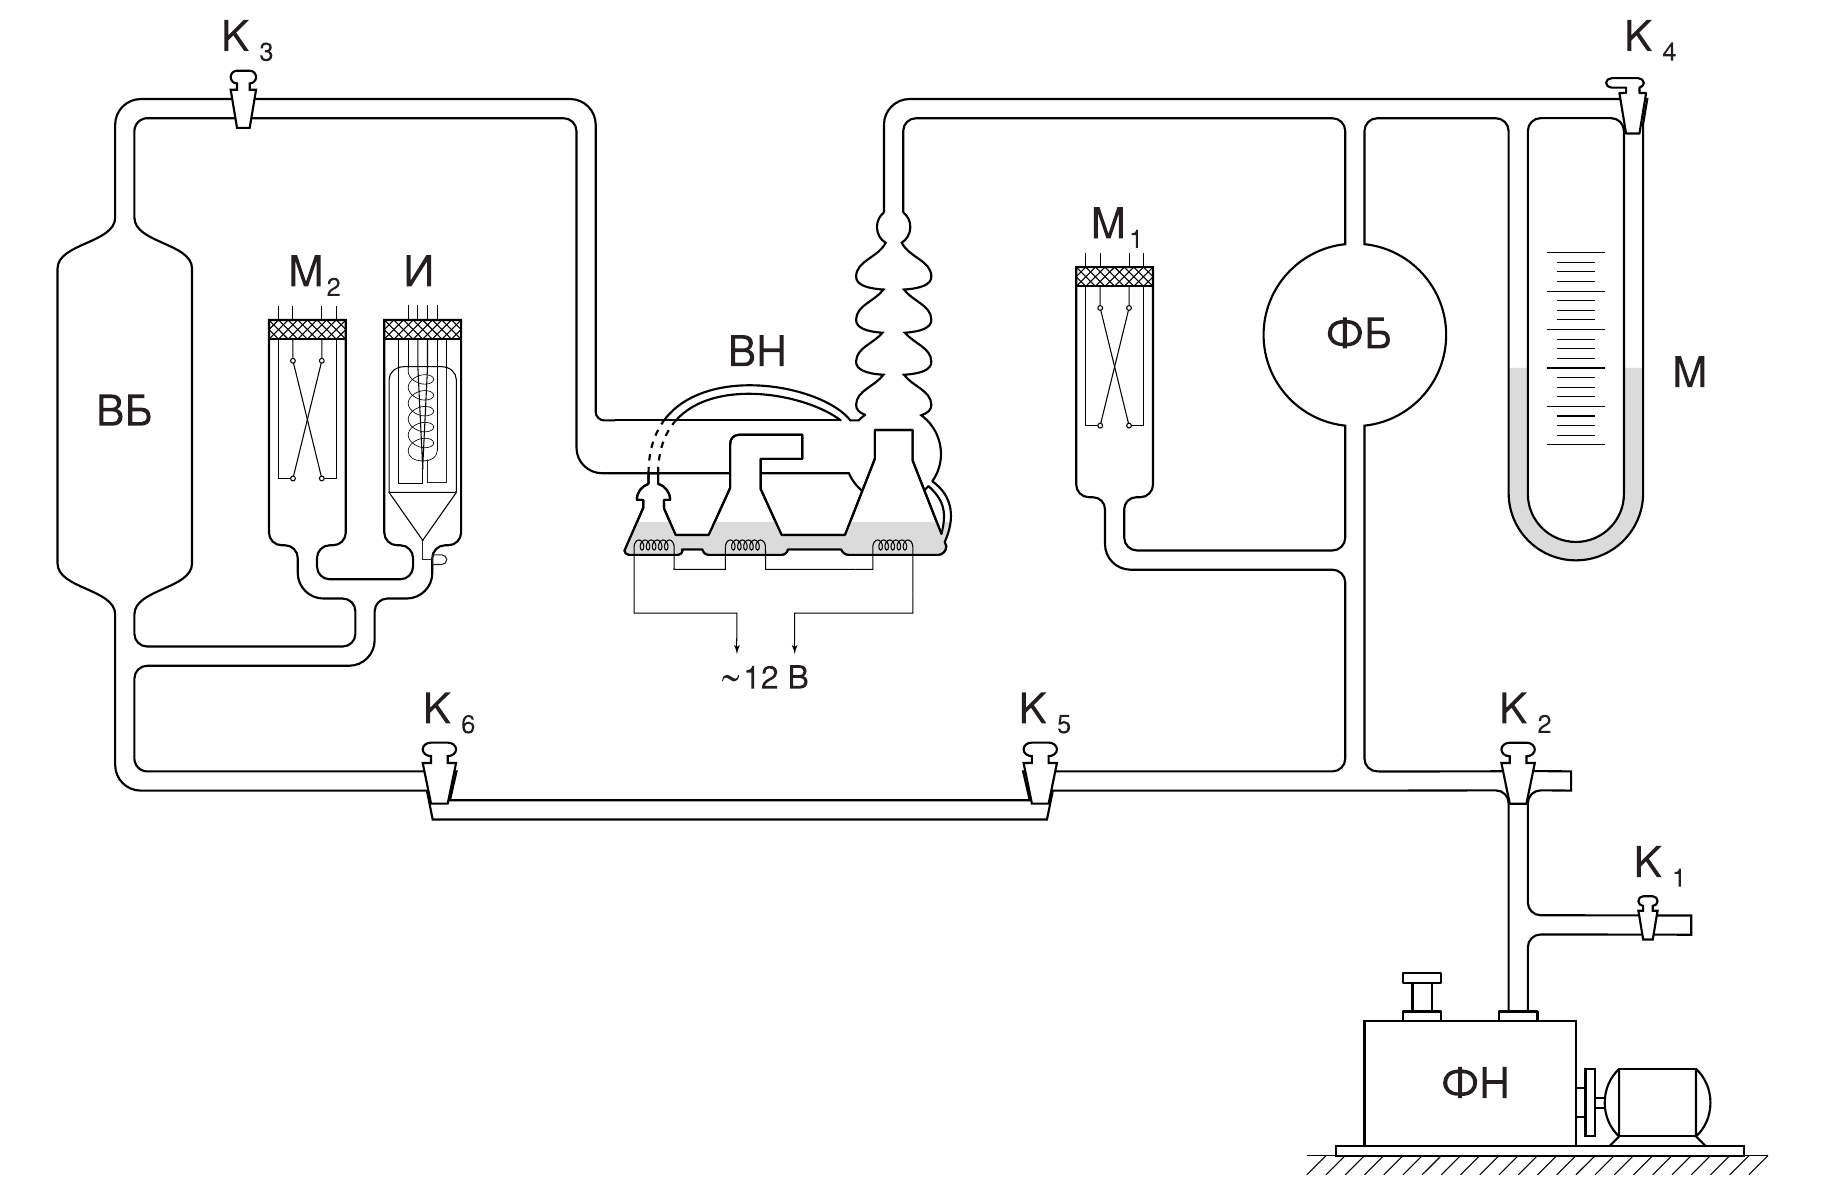
\includegraphics[width=0.9\textwidth]{data/установка.png}
  \end{center}
  \caption{Схема экспериментальной установки\label{fig:1}}
\end{figure}

Установка изготовлена из стекла и состоит из:
\begin{itemize}
  \item форвакуумного баллона (ФБ)
  \item высоковакуумного диффузионного насоса (ВН)
  \item высоковакуумного баллона (ВБ)
  \item масляного (М) и ионизационного (И) манометров
  \item термопарных манометров ($M_1$ и $M_2$)
  \item форвакуумного насоса (ФН)
  \item соединительных кранов ($K_1, \ldots, K_6$)
\end{itemize}

Все краны вакуумной установки стеклянные. Стенки кранов тонкие, пробки кранов полые и составляют одно целое с рукоятками.
Пробки кранов притерты к корпусам. Для герметизации используется вакуумная смазка.

\begin{figure} [H]
  \begin{center}
    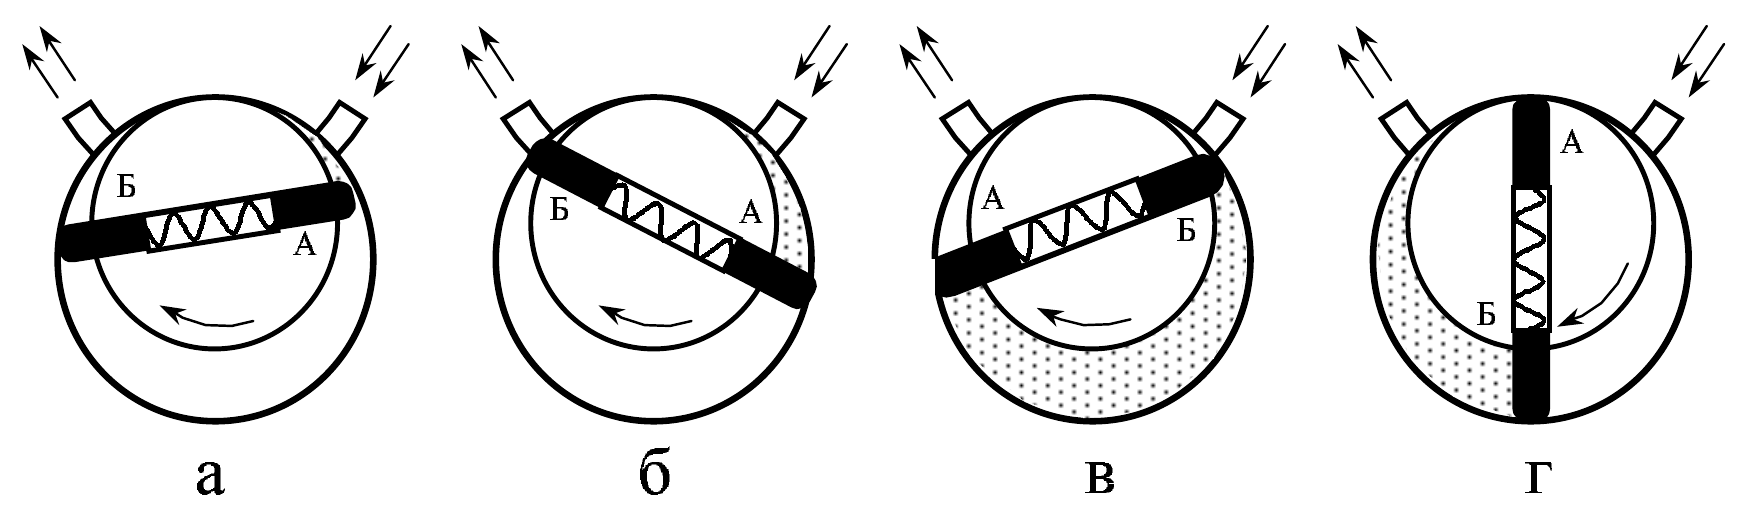
\includegraphics[width=0.9\textwidth]{data/ФН_принцип_работы.png}
  \end{center}
  \caption{Схема действия ФН.\label{fig:2}}
\end{figure}

Устройство и принцип действия \textit{форвакуумного насоса} схематически, но довольно ясно изображены на \figref{fig:2}.

\subsection{Диффузионный насос (ВН).}

\begin{figure} [H]
  \begin{center}
    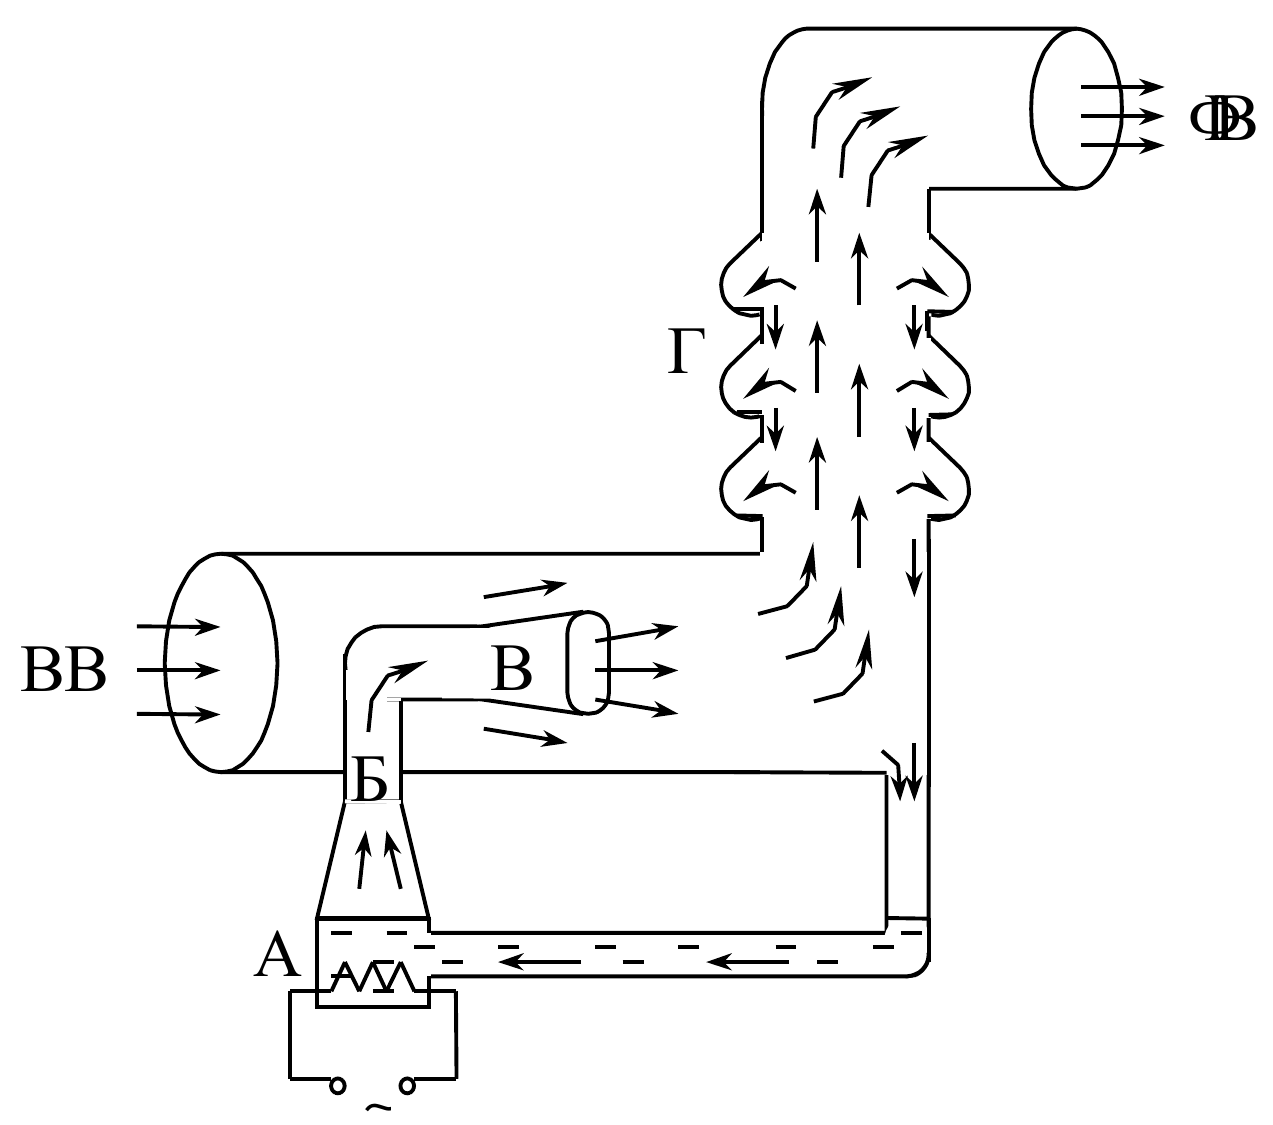
\includegraphics[width=0.7\textwidth]{data/ВН_принцип_работы.png}
  \end{center}
  \caption{Схема действия диффузионного насоса.\label{fig:3}}
\end{figure}

Масло, налитое в сосуд А, подогревается электрической печкой. Пары масла поднимаются по трубе Б и вырываются из сопла В.
Струя паров увлекает молекулы газа, которые поступают из откачиваемого сосуда через трубку ВВ.
Дальше смесь попадает в вертикальную трубу Г. Здесь масло осаждается на стенках трубы и маслосборников и стекает вниз, а оставшийся газ через трубу ФВ откачивается форвакуумным насосом.
Диффузионный насос работает наиболее эффективно при давлении, когда длина свободного пробега молекул воздуха
примерно равна ширине кольцевого зазора между соплом В и стенками трубы ВВ. В этом случае пары масла увлекают молекулы воздуха из всего сечения зазора.

Включать ВН стоит только при уже имеющемся вакууме $5 \cdot 10^{-2} \torr$.
После включения ВН, давление в системе сначала будет подниматся.
Через десять минут масло начнет испарятся, а ВН - работать.

\subsection{Масляный манометр (М).}
Две U-образные трубки, наполовину заполненные маслом.
Разница давления измеряется по разнице высот масла в двух трубках.

\begin{equation}
  \rho \approx 0.885\ \frac{\gr}{\cm^3}
  \label{val:rho}
\end{equation}
\begin{description}
  \item[$\rho$] - плотность масла в маслянном манометре.
\end{description}

\subsection{Термопарный манометр.}

% \begin{wrapfigure}{r}{50mm}
%   \begin{center}
%     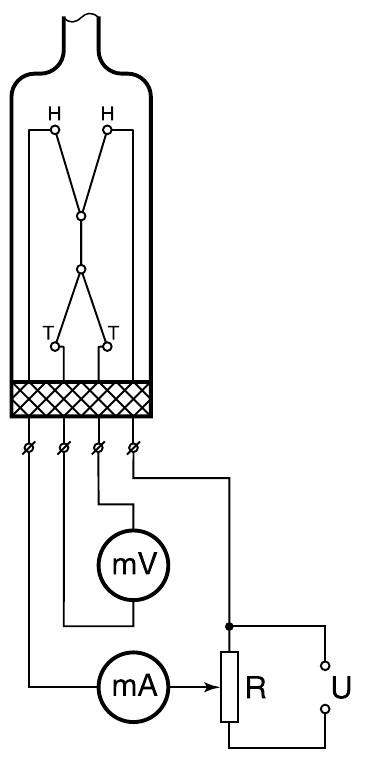
\includegraphics[width=0.9\linewidth]{data/ЛТ.png}
%     \caption{Схема термопарного манометра.\label{fig:Схема термопарного монометра}}
%   \end{center}
% \end{wrapfigure}

\seefigref{fig:Схема термопарного монометра}\\
По нити накала НН пропускается ток постоянной величины. Термопара ТТ присоединяется к милливольтметру,
показания которого определяются температурой нити накала и зависят от отдачи тепла вокружающее пространство.
Потери тепла определяются теплопроводностью нити и термопары, теплопроводностью газа, переносом тепла конвективными потоками газа внутри лампы и теплоизлучением нити (инфракрасноетепловое излучение).
В обычном режимелампы основную роль играет теплопроводность газа. При давлениях >1 торр теплопроводность газа, а вместе с ней и ЭДС термопары практически не зависят от давления газа,
и прибор не работает. При улучшении вакуума средний свободный пробег молекул становится сравнимым с диаметром нити, теплоотвод падает и температура спая возрастает. При вакууме $~10^{-3}$ торр
теплоотвод, осуществляемый газом, становится сравнимым с другими видами потерь теплаи температура
нити становится практически постоянной. \\
Градуировочная кривая термопарного манометра приведена на \seefigref{graph:M}.

\begin{figure}[H]
  \begin{minipage}{0.3\textwidth}
    \centering
    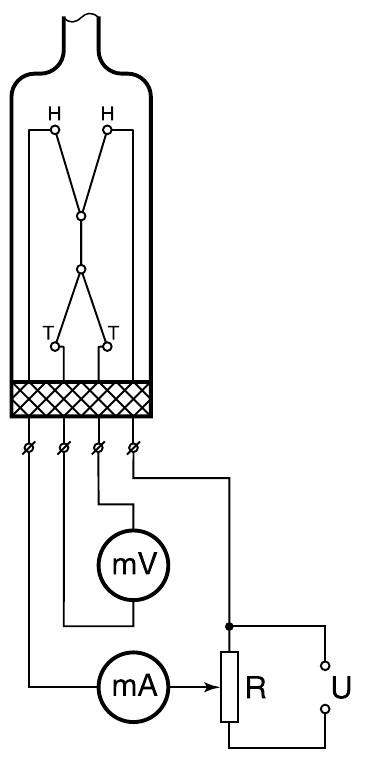
\includegraphics[width=0.9\linewidth]{data/ЛТ.png}
    \caption{Схема термопарного манометра.\label{fig:Схема термопарного монометра}}
  \end{minipage}\hfill
  \begin{minipage}{0.8\textwidth}
    \centering
    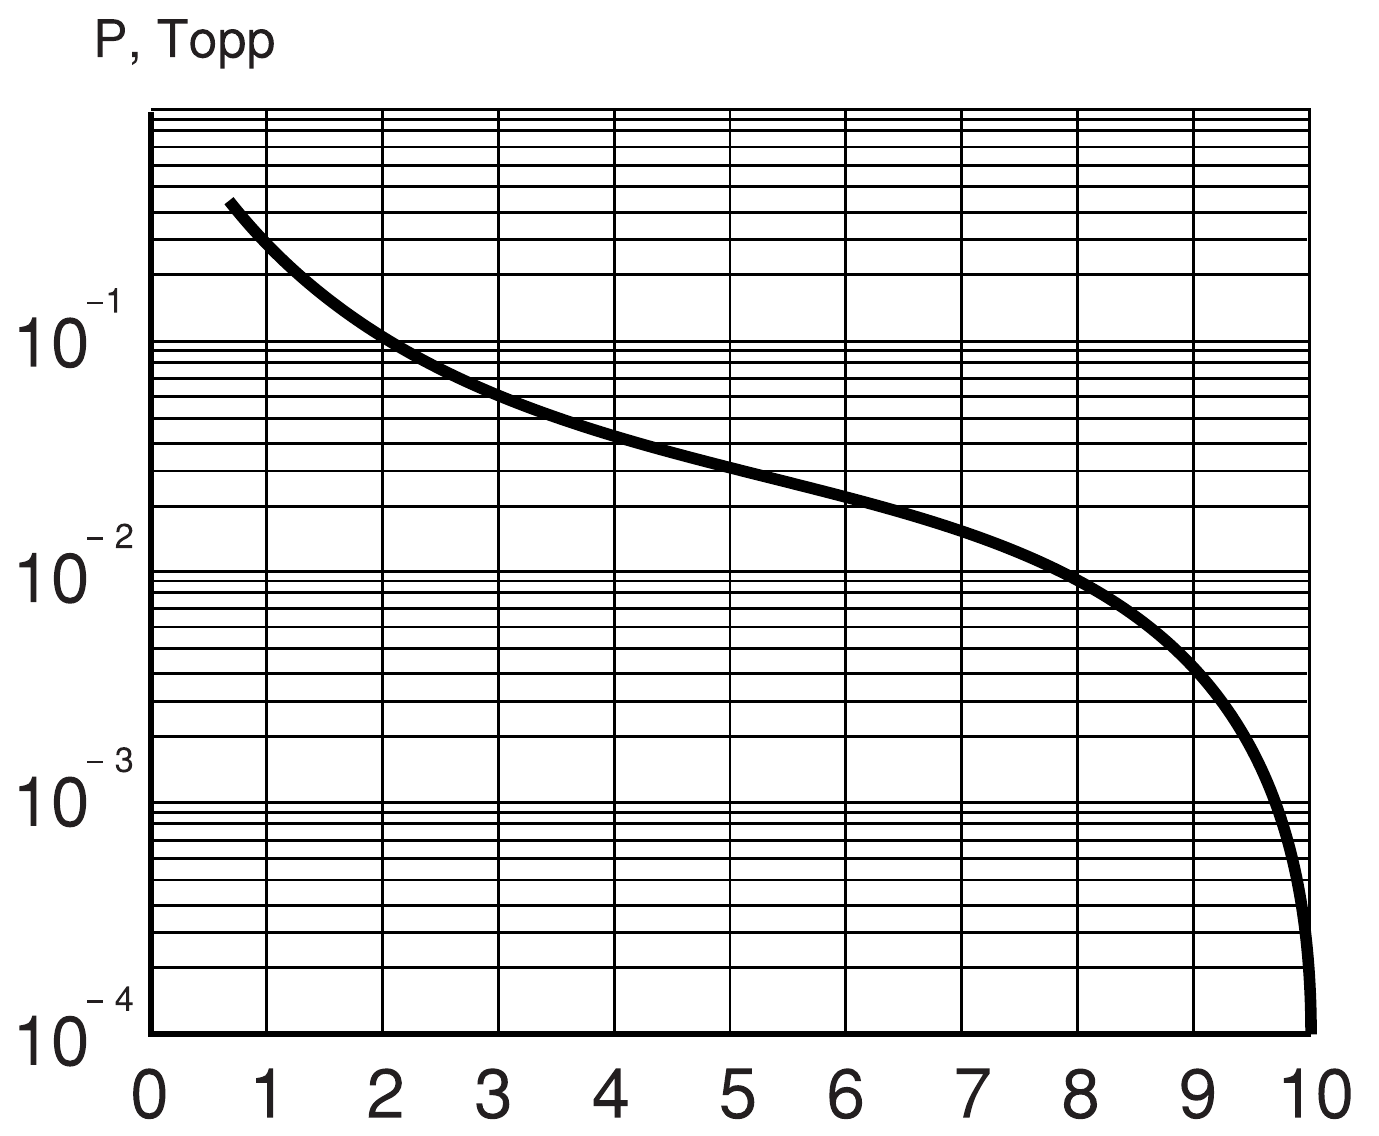
\includegraphics[width=0.8\textwidth]{data/ТМ_кривая.png}
    \caption{Градуировочная кривая термопары.\label{graph:M}}
  \end{minipage}\hfill
\end{figure}

\subsection{Ионизационный манометр.}
Схема ионизационного манометра изображена на \seefigref{fig:схема_ионизационной_лампы}.
Он представляет собой трехэлектродную лампу. Электроны испускаются накаленным катодом и увлекаются электрическим полем к аноду, имеющему вид спирали. Проскакивая за ее витки,электроны замедляются полем коллектора и возвращаются к катоду, а от него вновь увлекаются к аноду.
Прежде чем осесть на аноде, они успевают много раз пересечь пространство между катодом и коллектором.
На своем пути электроны ионизуют молекулы газа. Ионы, образовавшиеся между анодом и коллектором, притягиваются полем коллектора и определяют его ток.
Ионный ток в цепи коллектора пропорционален плотности газа и поэтому может служить мерой давления.
Вероятность ионизации зависит от рода газа, заполняющего лампу (а значит, и откачиваемый объем).
Калибровка манометра верна, если остаточным газом является воздух. Накаленный катод ионизационного манометра перегорает, если давление в системе превышает $10^{-3}$ торр.
Поэтому включать ионизационный манометр можно, только убедившись по термопарному манометру, что давление в системе не превышает $10^{-3}$ торр.
При измерении нить ионизационного манометра сильно греется. При этом она сама, окружающие ее электроды и стенки стеклянного баллона могут десорбировать поглощенные ранее газы.
Выделяющиеся газы изменяют давление в лампе и приводят к неверным показаниям. Поэтому перед измерениями ионизационный манометр прогревается (обезгаживается) в течение 10–15 мин. Для прогрева пропускается ток через спиральный анод лампы.

\begin{figure}[H]
  \centering
  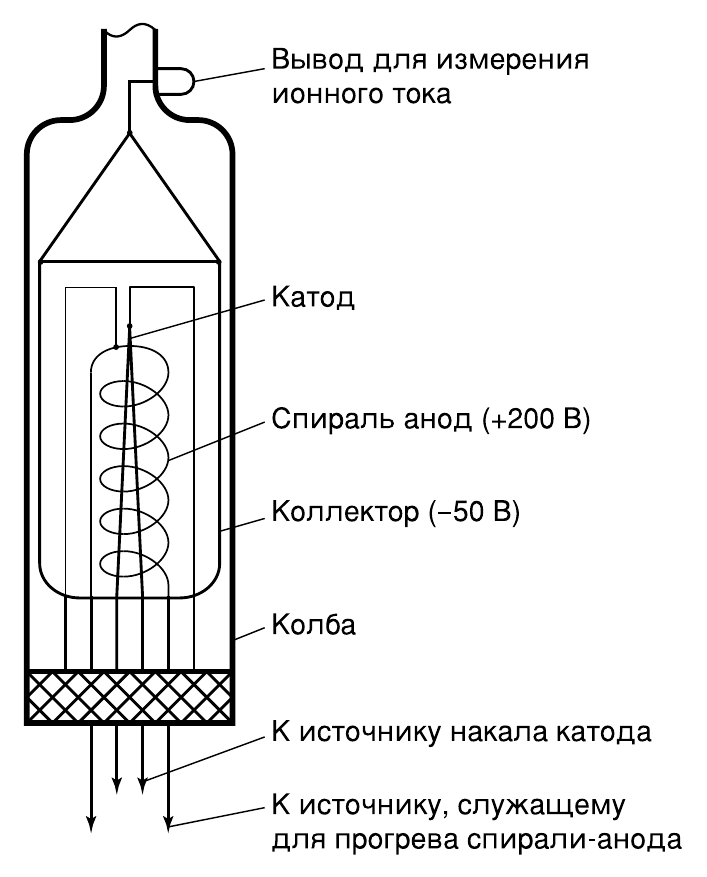
\includegraphics[width=0.5\textwidth]{6.png}
  \caption{Схема ионизационной лампы ЛМ-2.\label{fig:схема_ионизационной_лампы}}
\end{figure}

\section{Теоретическая часть}

\paragraph{Процесс откачки: }
Производительность насоса определяется скоростью откачки $W$ (л/с). Скорость откачки форвакуумного насоса равна емкости воздухозаборной камеры, умноженной на число оборотов в секунду.

Обозначим через $Q_\text{д}$ количество газа, десорбирующегося с поверхности откачиваемого объема в единицу времени,
$Q_\text{и}$ --- количество газа, проникающего в единицу времени в этот объем извне (через течи). \\
Будем считать, что насос обладает скоростью откачки $W$ и в то же время сам является источником газа. \\
Пусть $Q_\text{н}$ — поток газа, поступающего из насоса назад в откачиваемую систему. \\
Пусть $Q=Q_\text{д} + Q_\text{и} + Q_\text{н}$ (моль/с).

Получаем формулу:
\begin{equation}
  -V\d{P}=\left(P W - Q \cdot RT\right)\d{t}
\end{equation}

При предельном давлении $\d{P}=0$ и поэтому получаем:
\begin{equation}
  P_\text{пр} W = Q \cdot RT; \quad
  W = \frac{Q \cdot RT}{P_\text{пр}}
  \label{eq:2.2}
\end{equation}

Подставляя получаем
\begin{equation}
  -V\d{P}=W\left(P-P_\text{пр}\right)\d{t}
\end{equation}
Интегрируем полученное ур-е и получаем
\begin{equation}
  P-P_\text{пр}=(P_0 - P_\text{пр})\exp{\left(-\frac{W}{V}t\right)}
\end{equation}
% Пренебрегая $P_\text{пр}$ относитеьно $P_0$
\begin{equation}
  P=P_0\exp\left(-\frac{W}{V}t\right) + P_\text{пр}
  \label{eq:P(t)}
\end{equation}
Как видим, величина $\tau=V/W$ показывает характерное время откачки системы.

Теперь попробуем понять чем обусловлена скорость откачки. Очевидно, скорость $W$ зависит от скорости откачки насоса $W_\text{н}$, но она так же зависит от трубопровода соединяюшего насос к откачиваемой части, т.к. если трубопровод не сможет обеспечить достаточное количество газа к входу насоса то, производительность упадет.

Попробуем описать систему математически. Пусть у нас есть насос со скоростью откачки $W_\text{н}$ и трубопровод с пропускной способностью $C$. Давление в откачиваемом объеме -- $P_1$.

\begin{equation}
  C(P_1 - P_2)=W_\text{н} P_2 \implies
  P_2=\frac{CP_1}{C+W_\text{н}} \Rightarrow
  WP_1=W_\text{н} 2=\frac{C W_\text{н}}{C + W_\text{н}} P_1
\end{equation}
Как видим, для результирующей скорости $W$ верно соотношение

\begin{equation}
  \frac{1}{W} = \frac{1}{W_\text{н}} + \frac{1}{C}
\end{equation}
Обобщая это выражение для последовательно соединенных труб получаем

\begin{equation}
  \frac{1}{W} = \frac{1}{W_\text{н}} + \frac{1}{C_1} + \frac{1}{C_2} + ...
  \label{resulting_speed}
\end{equation}
Заметим только что данные формулировки верны при молекулярном режиме течения, когда вязкое трение не имеет большого вклада в движение газа.

\paragraph{Течение газа через трубу:} Для количества газa, протекающего через трубу в условиях высокого вакуума или, как говорят, в кнудсеновском режиме, справедлива формула (см. формулу 3.6):

\begin{equation}
  \frac{d(PV)}{\d{t}} = \frac{4}{3}r^3 \sqrt{\frac{2\pi RT}{\mu}} \frac{P_2 - P_1}{L}
  \label{eq:6}
\end{equation}

где $r$ и $L$ соответственно радиус и длина трубы. Если пренебречь давлением $P_1$ у конца, обращенного к насосу, получаем формулу для пропускной способности трубы
\begin{equation}
  C_\text{тр} = \frac{dV}{\d{t}} = \frac{4}{3}\frac{r^3}{L}\sqrt{\frac{2\pi RT}{\mu}}
\end{equation}
Для пропускной способности отверстия (например в кранах) имеем формулу

\begin{equation}
  C_\text{отв}=S\frac{\bar{v}}{4}
\end{equation}

\section{Ход работы}
\subsection{Определение объемов форвакуумной и высоковакуумной частей установки}
\begin{enumerate}
  \item Проверим, что кран К4 открыт. Откроем все краны, кроме К1 и К2.
  \item Впустим в установку атмосферный воздух через краны К1 и К2.
  \item Закроем краны К5 и К6.
        В этих кранах и соединяющем их капилляре «запирается» $V_\text{зап}$ воздуха при атмосферном давлении.
        \[V_\text{зап} = 50 \cm^3\]
  \item Закроем краны К1 и К2, включим ФН и дадим ему откачать себя. Подключим установку к ФН краном К2 и откачаем установку до давления $10^{-2}$ торр.
  \item Повернув рукоятку крана К2, отсоединим установку от ФН. Оставим ФН работать.
  \item Закроем К3.
  \item Закроем К4.
  \item Откроем К5.
  \item  Зная $V_\text{зап}$ (см. п. 3) и $\D{h_{1,2}}$, найдем, пользуясь законом Бойля–Мариотта, объем $V_\text{фв}$ форвакуумной части.
  Считаем, что объем труб мал, по сравнению с $V_\text{фв}$ и $V_\text{вв}$.
  \begin{equation}
    P_\text{атм} V_\text{зап} = P_1 V_\text{фв}
    \implies
    V_\text{фв} = \frac{P_\text{атм} V_\text{зап}}{P_1}
  \end{equation}
  \begin{equation}
    P = \rho g \D{h}. \quad~(\rho: ~\ref{val:rho})
  \end{equation}

  \[\D{h_1} = (25.3 \pm 0.1)\ \cm\]

  \begin{center}
    \fbox{
        \parbox{5cm}{
          \begin{center}
            $\D{h_1} = (25.3 \pm 0.1)\ \cm$ \\
            $P_1 = (18.6 \pm 1.9)\ \torr$ \\
            $V_\text{фв} = (2017 \pm 206)\ \cm^3$
          \end{center}
        }
    }
  \end{center}

  \item Откроем кран К3. \\
  Газ, занимавший $V_\text{фв}$, заполнит и высоковакуумную часть. Измерим показания манометра. Рассчитаем полный объем установки и объем высоковакуумной ее части $V_\text{вв}$.

  \begin{equation}
    P_\text{атм} V_\text{зап} = P_2 (V_\text{фв} + V_\text{вв})
    \implies
    V_\text{фв} = \frac{P_\text{атм} V_\text{зап}}{P_2} - V_\text{фв}
  \end{equation}

  \begin{center}
    \fbox{
        \parbox{5cm}{
          \begin{center}
            $\D{h_2} = (16.3 \pm 0.1)\ \cm$ \\
            $P_2 = (12.0 \pm 1.2)\ \torr$ \\
            $V_\text{вв} = (1113 \pm 380)\ \cm^3$
          \end{center}
        }
    }
  \end{center}

  \item Откроем K4.

  \item Повторим измерения 1 - 10 еще раз. \\
  Результат:
  \begin{center}
    \fbox{
        \parbox{5cm}{
          \begin{center}
            $\D{h_1} = (25.3 \pm 0.1)\ \cm$ \\
            $P_1 = (18.6 \pm 1.9)\ \torr$ \\
            $V_\text{фв} = (2017 \pm 206)\ \cm^3$
          \end{center}
        }
    }
  \end{center}

  \begin{center}
    \fbox{
        \parbox{5cm}{
          \begin{center}
            $\D{h_2} = (16.2 \pm 0.1)\ \cm$ \\
            $P_2 = (11.9 \pm 1.2)\ \torr$ \\
            $V_\text{вв} = (1133 \pm 382)\ \cm^3$
          \end{center}
        }
    }
  \end{center}

  Получили схожие значения.

\end{enumerate}

\subsection{Получение высокого вакуума и измерение скорости откачки}

\begin{enumerate}
  \item Откачаем установку с помощью ФН.

	\item Включим термопарные манометры, установим их токи согласно паспортам. Переключим прибор в режим измерения ЭДС и определим давление в установке по градуировочной кривой %\see_fig_ref{fig:5}

	\item По достижении форвакуума закрываем $K_6$ и начинаем откачку высоковакуумного баллона с помощью диффузионного насоса, для этого включаем нагреватель масла в ВН и ждем 10 минут, пока масло не начнет испарятся.\\

	\item Включим ионизационный манометр. Воспользуемся инструкцией.

	\item Измерим предельное давление $P_\text{пр}$ в системе.\\
	\begin{center}
    \fbox{$P_\text{пр} \approx 9.7 \cdot 10^{-5}\ \torr \approx 0.013\ \Pa$}
  \end{center}

  \item Измерим скорость ухудшения и улучшения вакуума.
  \begin{enumerate}
    \item Закроем К3.\\
    Из за течей, Вакуум в ВБ начнет ухудшаться, а давление P --- возрастать.
    \item Измерим зависимасть P на ионизационном манометре от времени (см. т. \ref{table:first_devacuuming}).\\
    Изобразим результаты на графике (см. рис. \ref{plot:first_devacuuming}).
    \item Когда P станет равным $(5-9)\cdot 10^{-4}\ \Pa$, откроем К3.\\
    Вакуум в ВБ начнет улучшаться, а давление P --- убывать.
    \item Измерим зависимасть P на ионизационном манометре от времени (см. т. \ref{table:first revacuuming}).\\
    Изобразим результаты на графике (см. рис. \ref{plot:first_revacuuming}).
  \end{enumerate}
  Расчитаем W по наклону линий тренда на графиках \ref{plot:first_revacuuming} и \ref{plot:second_revacuuming}.\\
  Пусть наклон --- $\alpha$, тогда по ур-ию \eqref{eq:P(t)}:
  \begin{equation}
    W = -\alpha \cdot V
  \end{equation}
  \begin{description}
    \item[V] --- откачиваемый объем
  \end{description}

  \begin{center}
    \fbox{
      \parbox{7cm}{
        \begin{center}
          $\alpha_2 = (-0.202 \pm 0.004)\ 1 / \sec$ \\
          $\alpha_4 = (-0.195 \pm 0.003)\ 1 / \sec$ \\
          $\avrg{\alpha} = (-0.199 \pm 0.004)\ 1 / \sec$
        \end{center}
      }
    }
  \end{center}

  \begin{center}
    \fbox{
      \parbox{7cm}{
        \begin{center}
          $\avrg{W} = (223 \pm 76)\ \ml / \sec$\label{W1}
        \end{center}
      }
    }
  \label{value: W_2}
  \end{center}


  \item Оценим $Q_\text{н}$.

  Для этого воспользуемся полученными даннимы при ухудшении вакуума.\\
  (см. таблицу \ref{table:1 and 2}, см. графики (\ref{plot:first_devacuuming}, \ref{plot:second_devacuuming}))

  В данном процессе справидлива следующая формула:
  \begin{equation}
    V_\text{вв} \d{P} = (Q_\text{д} + Q_\text{и}) \d{t}
  \end{equation}
  
  Также воспользуемся \eqref{eq:2.2}.

  Получим:
  \begin{equation}
    Q_\text{н} = \frac{1}{RT} (P_\text{пр} W - V_\text{вв} \deriv{P}{t})
  \end{equation}

  \begin{center}
    \fbox{
      \parbox{7cm}{
        \begin{center}
          $Q_\text{н} = (-3.336 \pm 3.291)\ \mol/\sec$\label{Qn}
        \end{center}
      }
    }
  \end{center}
  
	\item Проведем измерения 6 - 7 еще раз.
	
  \item Откроем кран К6. Вакуум в установке должен ухудшиться. Измерим установившееся давление $P_\text{уст}$ и давление со стороны форвакуумной части капилляра.
  
  \begin{center}
    \fbox{
      \parbox{5cm}{
        \begin{center}
          $P_\text{уст} \approx 2.3 \cdot 10^{-4}\ \torr$ \\
          $P_\text{фв} \approx 1 \cdot 10^{-4}\ \torr$
        \end{center}
      }
    }
  \end{center}

  \item Рассчитаем производительность насоса по различию $P_\text{уст}$ и $P_\text{пр}$. Для этого найдите количество газа, протекающего через капилляр, по
  
  \begin{equation}
    P_\text{пр}W = Q_1, \quad
    P_\text{уст}W = Q_1 + \frac{\d{(PV)_{\text{капилляр}}}}{\d{t}}
  \end{equation}

  По формуле~\eqref{eq:6}:

  \begin{equation}
    (P_\text{уст} - P_\text{пр})W = 
    \frac{4}{3}(d/2)^3\sqrt{\frac{2\pi RT}{\mu}}\frac{P_\text{фв}}{L}
  \end{equation}

  \begin{center}
    \fbox{
      $
      W = (4.12 \pm 1.97) \cdot 10^{-7}\ \m^3 / \sec =
      (0.412 \pm 0.197)\ \ml / \sec
      $\label{W2}
    }
  \end{center}
  \begin{center}
    \fbox{
      $\eps_W \approx 48\%$~!?!
    }
  \end{center}

  \item Выключим установку.

\end{enumerate}

\begin{table}[H]
  \begin{minipage}[t]{.45\linewidth}
    \begin{center}
    \begin{tabular}{c|cc}
    &t, с&P, $\torr \cdot 10^{-5}$\\
    \hline
    0&22.06&11\\
    1&25.07&12\\
    2&26.19&13\\
    3&27.18&14\\
    4&29.04&15\\
    5&30.03&16\\
    6&31.04&17\\
    7&32.22&18\\
    8&33.22&19\\
    9&35.06&20\\
    10&36.16&21\\
    11&37.22&22\\
    12&39.03&23\\
    13&40.03&24\\
    14&41.22&25\\
    15&43.15&26\\
    16&44.04&27\\
    17&45.21&28\\
    18&47.04&29\\
    19&48.04&30\\
    20&49.16&31\\
    21&51.07&32\\
    22&52.18&33\\
    23&53.22&34\\
    24&55.04&35\\
    25&56.18&36\\
    26&58.04&37\\
    27&59.04&38\\
    28&60.19&39\\
    29&62.03&40\\
    30&63.24&41\\
    31&64.21&42\\
    32&66.09&43\\
    33&67.21&44\\
    34&69.06&45\\
    35&70.21&46\\
    36&72.06&47\\
    37&73.19&48\\
    38&74.25&49\\
    39&76.09&50\\
    40&77.21&51\\
    41&79.06&52\\
    42&80.18&53\\
    43&82.03&54\\
    44&83.21&55\\
    45&85.04&56\\
    46&86.18&57\\
    47&87.19&58\\
    48&89.06&59\\
    49&90.21&60\\
    50&92.04&61\\
    51&93.21&62\\
    \end{tabular}
    \end{center}
    \caption{first devacuuming\label{table:first_devacuuming}}
  \end{minipage}
  \begin{minipage}[t]{.45\linewidth}%\vspace{0pt}
    \begin{center}
    \begin{tabular}{c|cc}
    &t, с&P, $\torr \cdot 10^{-5}$\\
    \hline
    0&169.02&12\\
    1&171.16&13\\
    2&173.01&14\\
    3&174.02&15\\
    4&175.18&16\\
    5&176.16&17\\
    6&178.01&18\\
    7&178.3&19\\
    8&180.15&20\\
    9&181.15&21\\
    10&182.3&22\\
    11&183.3&23\\
    12&185.15&24\\
    13&186.18&25\\
    14&188.03&26\\
    15&189.02&27\\
    16&190.16&28\\
    17&191.3&29\\
    18&193.04&30\\
    19&194.17&31\\
    20&196.05&32\\
    21&197.01&33\\
    22&198.15&34\\
    23&200.01&35\\
    24&201.02&36\\
    25&202.16&37\\
    26&204.04&38\\
    27&205.01&39\\
    28&206.17&40\\
    29&207.3&41\\
    30&209.16&42\\
    31&210.3&43\\
    32&211.3&44\\
    33&213.16&45\\
    34&215.02&46\\
    35&216.17&47\\
    36&217.18&48\\
    37&219.01&49\\
    38&220.16&50\\
    39&222.01&51\\
    40&223.16&52\\
    41&224.3&53\\
    42&226.15&54\\
    43&227.15&55\\
    44&229.01&56\\
    45&230.15&57\\
    46&232.01&58\\
    47&233.15&59\\
    48&234.3&60\\
    49&236.01&61\\
    50&237.18&62\\
    \end{tabular}
    \end{center}
    \caption{second devacuuming\label{table:second devacuuming}}
  \end{minipage}
  \caption{Данные зависимости давления от времени при ухудшении вакуума (см. пункт 6 выполнения).\label{table:1 and 2}}
  \end{table}
  
  \begin{table}[H]
  \begin{minipage}[t]{.4\linewidth}%\vspace{0pt}
    \begin{center}
    \begin{tabular}{c|cc}
    &t, с&P, $\torr \cdot 10^{-5}$\\
    \hline
    0&237.18&62\\
    1&238.17&61\\
    2&239.17&60\\
    3&240.03&58\\
    4&240.18&56\\
    5&241.02&53\\
    6&241.17&49\\
    7&242.02&46\\
    8&242.17&43\\
    9&243.03&39\\
    10&243.18&36\\
    11&244.02&33\\
    12&244.16&31\\
    13&245.04&28\\
    14&245.16&26\\
    15&246.03&25\\
    16&246.17&23\\
    17&247.02&22\\
    18&247.16&21\\
    19&248.01&20\\
    20&248.17&19\\
    21&249.04&18\\
    22&249.15&17\\
    23&250.17&16\\
    24&251.15&15\\
    25&253.02&14\\
    26&254.18&13\\
    27&257.02&12\\
    28&264.02&11\\
    \end{tabular}
    \end{center}
    \caption{first revacuuming\label{table:first revacuuming}}
  \end{minipage}
  \begin{minipage}[t]{.4\linewidth}%\vspace{0pt}
    \begin{center}
    \begin{tabular}{c|cc}
      &t, с&P, $\torr \cdot 10^{-5}$\\
      \hline
      0&93.21&62\\
      1&95.04&61\\
      2&96.02&59\\
      3&96.16&57\\
      4&97.01&54\\
      5&97.17&51\\
      6&98.02&47\\
      7&98.16&43\\
      8&99.02&40\\
      9&99.17&36\\
      10&100.02&33\\
      11&100.17&30\\
      12&101.01&28\\
      13&101.16&26\\
      14&102.01&24\\
      15&102.17&23\\
      16&103.01&21\\
      17&103.18&20\\
      18&104.02&19\\
      19&105.02&18\\
      20&105.17&17\\
      21&106.01&16\\
      22&107.01&15\\
      23&108.16&14\\
      24&110.02&13\\
      25&113.02&12\\
      26&117.01&11\\
    \end{tabular}
    \end{center}
    \caption{second revacuuming\label{table:second revacuuming}}
  \end{minipage}
  \caption{Данные зависимости давления от времени при улучшении вакуума (см. пункт 6 выполнения).\label{table:3 and 4}}
  \end{table}
  
  \begin{figure} [H]
    \centering
    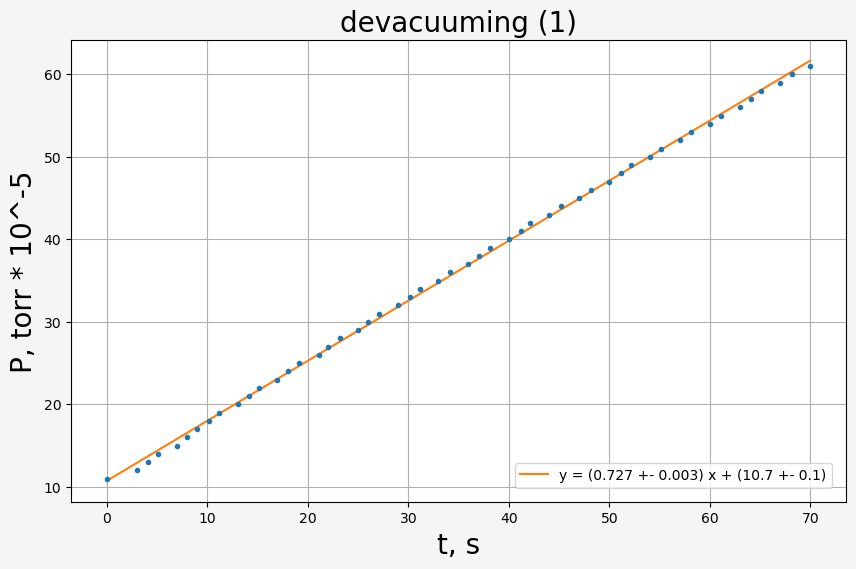
\includegraphics[scale=0.8]{plot1.png}
    \caption{График зависимости давления от времени при ухудшении вакуума (1).
  ~\label{plot:first_devacuuming}}
  \end{figure}
  
  \begin{figure} [H]
    \centering
    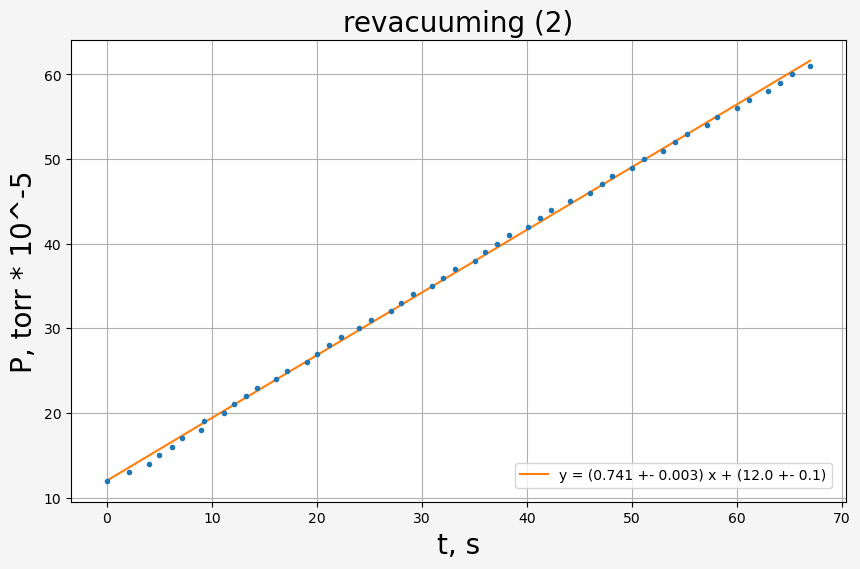
\includegraphics[scale=0.8]{plot2.png}
    \caption{График зависимости давления от времени при улучшении вакуума (1).
  ~\label{plot:first_revacuuming}}
  \end{figure}
  
  \begin{figure} [H]
    \centering
    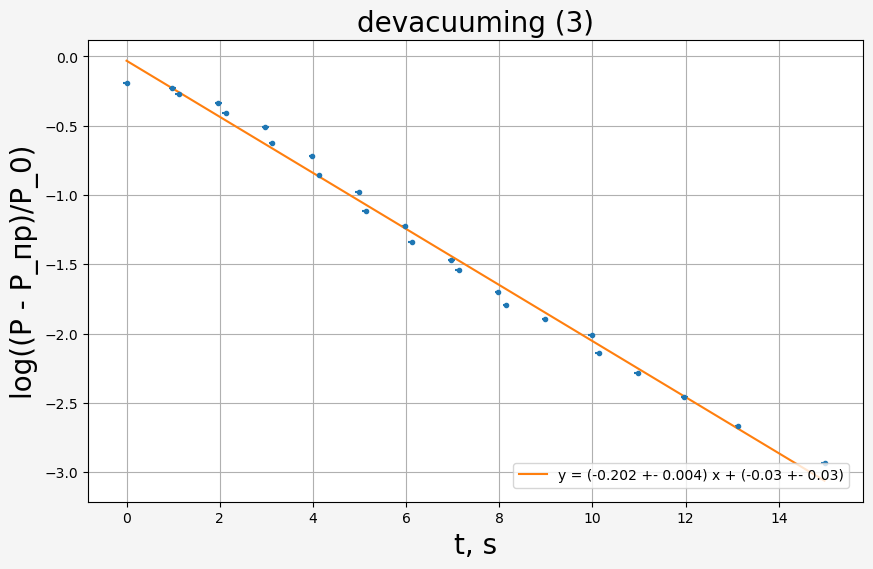
\includegraphics[scale=0.8]{plot3.png}
    \caption{График зависимости давления от времени при ухудшении вакуума (2).
  ~\label{plot:second_devacuuming}}
  \end{figure}
  
  \begin{figure} [H]
    \centering
    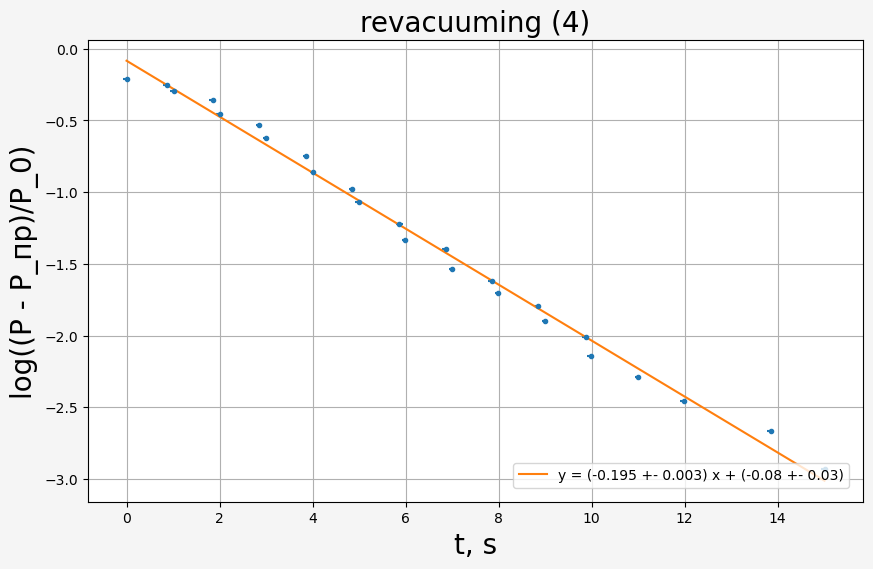
\includegraphics[scale=0.8]{plot4.png}
    \caption{График зависимости давления от времени при улучшении вакуума (2).
  ~\label{plot:second_revacuuming}}
  \end{figure}

\section{Вывод.}
В результате лабораторной работы мы нашли объемы форвакуумной и высоковакуумной частей установки. Определили скорости ухудшения и улучшения вакуума по зависимостям P(t) (см. графики и таблицы).\\

Нашли W двумя способами.\\
МНК: \ref{W1}\\
По ф-ле Кнудсена: \ref{W2}\\

Значения получились совершенно разные 


Нашли $Q_\text{н}$. \ref{Qn}\\


\end{document}
